\chapter{Conversores CC com Cargas de Potência Constante} \label{cap3}

\section{Microrredes CC}

No século XX, a "Guerra das Correntes" entre defensores da \acrshortpl{ca}, liderados por \textit{Westinghouse} e \textit{Tesla}, e proponentes da \acrshort{cc}, liderados por \textit{Edison}, resultou na prevalência da \acrshort{ca} devido à sua facilidade de expansão da rede. Apesar disso, a \acrshort{cc} permaneceu relevante com os avanços na eletrônica de potência. Paralelamente, a crescente adoção de microrredes \acrshortpl{mr}, com \acrfullpl{fer}, \acrfullpl{sae} e novas cargas, reflete preocupações ambientais e escassez de combustíveis fósseis, mas sua integração descoordenada apresenta desafios técnicos e operacionais, como perfil de tensão comprometido e congestionamentos nas linhas de transmissão. \cite{Elsayed2015, Dragicevic2015}.

A proposta das \acrshortpl{mr} surgiu como uma solução há mais de uma década. As \acrshortpl{mr}, operando em modo isolado ou conectadas à rede, podem ser classificadas como \acrshortpl{mr} de \acrshort{ca} ou \acrshort{cc}, sendo a \acrshort{mr} de \acrshort{cc} mais atraente devido à sua maior eficiência e melhor interface com diversos tipos de \acrshort{fer} e \acrshort{sae}. Além disso, ao serem acopladas em torno de um barramento \acrshort{cc}, as \acrfullpl{mr} eliminam problemas como fluxo de potência reativa e regulação de frequência, resultando em sistemas de controle menos complexos. \cite{Dragicevic2015}.

Vários setores empregam \acrfullpl{sdcc}, como espaçonaves, centros de dados, telecomunicações, tração e sistemas de energia a bordo de navios. Por exemplo, a Estação Espacial Internacional utiliza \acrshortpl{sdcc} para operar suas vastas necessidades de energia. Alguns centros de dados também adotaram sistemas \acrshort{cc}, resultando em economia significativa de energia em comparação com sistemas \acrshort{ca} tradicionais. Na área de telecomunicações, os sistemas de distribuição de energia de 48V são amplamente empregados para garantir alta confiabilidade e eficiência. Além disso, sistemas de tração, como bondes e metrôs, preferem distribuição \acrshort{cc} devido à facilidade de interface com motores \acrshort{cc}. Esses sistemas também permitem maior eficiência e controlabilidade. Em sistemas de energia a bordo de navios, a distribuição zonal \acrshort{cc} é uma opção popular devido à sua confiabilidade e facilidade de proteção. \cite{Elsayed2015}.

Desta forma, o design de sistemas de distribuição \acrshort{cc} tem recebido atenção crescente, especialmente devido a adaptação de equipamentos projetados originalmente para \acrshort{ca}. Modelos simplificados são essenciais para compreender o comportamento da carga em operação \acrshort{cc}. Comparando configurações de cabos, descobriu-se que sistemas \acrshort{cc} podem superar \acrshort{cc} em termos de capacidade de transferência de energia, \cite{Salomonsson2007}. Em um estudo sobre microrredes \acrshort{cc} em centros de dados, \cite{Salomonsson2008}, foi proposto um sistema de controle adaptativo para otimizar o fluxo de energia e minimizar perdas. A coordenação entre conversores é crucial para garantir o fornecimento contínuo de energia às cargas sensíveis. Essas pesquisas contribuem para uma compreensão mais profunda do design e controle de sistemas de distribuição DC.

\section{Conversores CC e Cargas de Potência Constante}



\section{Modelagem Matemática}

% Introdução
% To-do: não esquecer de apresentar a forma completa da CPL
Nesta seção, aprofundaremos na modelagem matemática de uma microrrede, concentrando em um conversor buck operando em conjunto com uma \acrshort{cpl}. O conversor buck assume um papel fundamental na conversão de alta para baixa tensão contínua, enquanto a \acrshort{cpl} representa um tipo de carga com uma demanda de potência invariável, mesmo diante de flutuações na tensão de entrada. Essa análise aprofundada tem como objetivo desvendar os princípios basilares que regem essa configuração específica da microrrede, lançando as bases para análises subsequentes e o desenvolvimento de estratégias de controle eficazes.

Para facilitar cálculos e análises, este sistema simplificado será composta por um conversor buck e a \acrshort{cpl} será modelada como uma fonte de corrente, como apresentado na \autoref{fig:circuit1}. Essa modelagem captura o comportamento essencial que permite o estudo aprofundado das estratégias de \acrshort{etc} para conversores \acrshort{cc}. No circuito apresentado, os componentes incluem resistores ($R_L$, $R_C$), um capacitor ($C$) e um indutor ($L$). O parâmetro $d$ representa o \textit{duty cycle}, enquanto $I_{\acrshort{cpl}}$ indica a corrente da \acrshort{cpl}. Além disso, são observadas as tensões de entrada ($V_{in}$) e saída ($V_{out}$). Esses elementos desempenham papéis essenciais na operação e caracterização do circuito em questão, contribuindo para a compreensão abrangente de seu funcionamento e comportamento.

\begin{figure}[H]
  \centering
  % \vspace{3ex}
  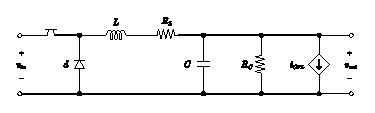
\includegraphics[scale=2.5]{figuras/buck_conversor_with_cpl_circuit.eps}
  \caption{Circuito \textit{Buck} com \acrshort{cpl}.}
  \label{fig:circuit1}
\end{figure}

% Introdução para o desenvolvimento das equações
% To-do: não esquecer de apresentar a forma completa do MMS e do MPS
% Dúvida: É para ser mais detalhista na obtenção das equações?
As equações que regem o comportamento do sistema são derivadas das leis fundamentais da eletricidade. O modelo matemático do conversor \textit{buck} se baseia no \acrshort{mms}. Apesar da natureza não linear intrínseca dos conversores, a prática usual é empregar \acrshort{mps} para obter uma representação linearizada em torno do ponto de operação. Para tal, o circuito é analisado em duas situações distintas: chave fechada e chave aberta.

% Modelagem do sistema para chave fechada
Na situação em que a chave está fechada, o circuito pode ser simplificado para um circuito série composto por uma fonte de tensão, um resistor e uma indutância, como ilustrado na \autoref{fig:circuit2}.

\begin{figure}[H]
  \centering
  % \vspace{3ex}
  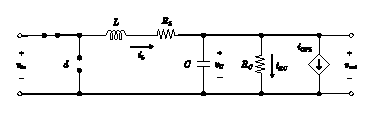
\includegraphics[scale=2.5]{figuras/buck_conversor_with_cpl_circuit_m1.eps}
  \caption{Circuito com a chave fechada.}
  \label{fig:circuit2}
\end{figure}

\noindent As equações que descrevem esse circuito são apresentadas abaixo:
% Lembrança: Faltou explica o que seria a Pcpl

\begin{equation}
  \begin{cases}
    \frac{d}{dt}i_L =  \frac{1}{L} V_{in}  - \frac{R_L}{L} i_L - \frac{1}{L} v_C \\
    \frac{d}{dt} v_C = \frac{1}{C} i_L - \frac{1}{C R_C} v_C - \frac{1}{C v_C} P_{CPL}
    \label{eq:circuito-m1}
  \end{cases}
\end{equation}
\\
\indent Na segunda situação, a chave está aberta e, consequentemente, a fonte de tensão é desconectada do circuito. Essa situação é representada na \autoref{fig:circuit3}.

\begin{figure}[H]
  \centering
  % \vspace{3ex}
  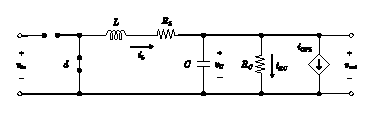
\includegraphics[scale=2.5]{figuras/buck_conversor_with_cpl_circuit_m2.eps}
  \caption{Circuito com a chave aberta.}
  \label{fig:circuit3}
\end{figure}

Neste caso, as equações que descrevem o circuito quando a chave está aberta são:

\begin{equation}
  \begin{cases}
    \frac{d}{dt}i_L  & = \frac{V_{in}}{L} d - \frac{R_L}{L} i_L - \frac{1}{L} v_C        \\
    \frac{d}{dt} v_C & = \frac{1}{C} i_L - \frac{1}{C R_C} v_C - \frac{1}{C v_C} P_{CPL}
    \label{eq:circuito-m2}
  \end{cases}
\end{equation}
\\
A partir da \autoref{eq:circuito-m1} e \autoref{eq:circuito-m2}, derivadas anteriormente, podemos estabelecer as seguintes equações diferenciais, as quais caracterizam o \acrshort{mms} e fornecem uma descrição do comportamento do circuito durante a operação contínua da chave.

\begin{equation}
  \begin{cases}
    \frac{d}{dt}i_L  & = \frac{V_{in}}{L} d - \frac{R_L}{L} i_L - \frac{1}{L} v_C        \\
    \frac{d}{dt} v_C & = \frac{1}{C} i_L - \frac{1}{C R_C} v_C - \frac{1}{C v_C} P_{CPL}
    \label{eq:nonlinear-system}
  \end{cases}
\end{equation}
\\
\indent Por meio da \autoref{eq:nonlinear-system}, onde é apresentado o sistema não linear, pode-se obter o sistema linearizado em torno dos pontos de operação. Esse sistema linear é representado por um conjunto de equações diferenciais, que descrevem as variações no tempo das grandezas $\delta i_L$ e $\delta v_C$, representando as alterações na corrente do indutor e na tensão do capacitor, respectivamente.

Considerando o sistema linearizado descrito por: \begin{equation} \dot{x} = Ax(t) + B_uu(t) + B_ww(t), \end{equation} onde  $x = \begin{bmatrix} \delta i_L & \delta v_C \end{bmatrix} ^ T$ representa o estado do sistema, $u = \delta d$ é a entrada do sistema e $w = \delta P_{CPL}$ é o sinal de pertubação. Além disto, $A \in \mathbb{R}^{n \times n}$, $B_u \text{ e } B_w \in \mathbb{R}^{n \times 1}$, são obtidos por meio das matrizes jacobianas das equações em (\ref{eq:nonlinear-system}), em torno do ponto de equilíbrio $P_{eq} = ({i_L}_0, \hspace{0.07cm} {v_C}_0, \hspace{0.07cm} {d}_0, \hspace{0.07cm} {P_{CPL}}_0)$. Portanto, o sistema linearizado obtido pode ser expresso como:

\begin{equation}
  \begin{bmatrix}
    \dot{\delta i_L} \\ \dot{\delta v_C}
  \end{bmatrix}
  =
  \begin{bmatrix}
    -\frac{R_L}{L} & -\frac{1}{L}                                                                \\
    \frac{1}{C}    & \frac{1}{C}\left(\frac{{P_{CPL}}_0}{{{{v_{C}}_0}^2}} - \frac{1}{R_C}\right)
  \end{bmatrix}
  \begin{bmatrix}
    \delta i_L \\ \delta v_C
  \end{bmatrix}
  +
  \begin{bmatrix}
    {\frac{V_{in}}{L}} & 0                     \\
    0                  & {-\frac{1}{C{v_C}_0}}
  \end{bmatrix}
  \begin{bmatrix}
    \delta d \\ \delta P_{CPL}
  \end{bmatrix}
\end{equation}

\section{Simulação}
